% \documentclass[acmtog,anonymous,review]{acmart}
% \acmSubmissionID{1234}
\documentclass[acmtog,review]{acmart}


\usepackage{booktabs} % For formal tables
\usepackage{xcolor}

% TOG prefers author-name bib system with square brackets
\citestyle{acmauthoryear}
%\setcitestyle{nosort,square} % nosort to allow for manual chronological ordering



\usepackage[ruled]{algorithm2e} % For algorithms
\renewcommand{\algorithmcfname}{ALGORITHM}
\SetAlFnt{\small}
\SetAlCapFnt{\small}
\SetAlCapNameFnt{\small}
\SetAlCapHSkip{0pt}

% Metadata Information
\acmJournal{TOG}
%\acmVolume{38}
%\acmNumber{4}
%\acmArticle{39}
%\acmYear{2019}
%\acmMonth{7}

% Copyright
%\setcopyright{acmcopyright}
%\setcopyright{acmlicensed}
%\setcopyright{rightsretained}
%\setcopyright{usgov}
%\setcopyright{usgovmixed}
%\setcopyright{cagov}
%\setcopyright{cagovmixed}

% DOI
%\acmDOI{0000001.0000001_2}

% Paper history
%\received{February 2007}
%\received{March 2009}
%\received[final version]{June 2009}
%\received[accepted]{July 2009}



% Document starts
\begin{document}

% Title portion
\title{Single-view TSDF Mesh Noise Reduction under Virtual Light Using Differentiable Rendering}

% DO NOT ENTER AUTHOR INFORMATION FOR ANONYMOUS TECHNICAL PAPER SUBMISSIONS TO SIGGRAPH 2019!
\author{PilJoong Jeong}
\orcid{0000-0001-7579-2047}
\affiliation{
 \institution{Gwangju Institute of Science and Technology}
 \streetaddress{123 Cheomdangwagi-ro}
 \city{Buk-gu}
 \state{Gwangju}
 \postcode{61005}
 \country{Republic of Korea}}
\email{piljoong.jeong@gm.gist.ac.kr}

%\renewcommand\shortauthors{Jeong, P. et al}

\begin{teaserfigure}
    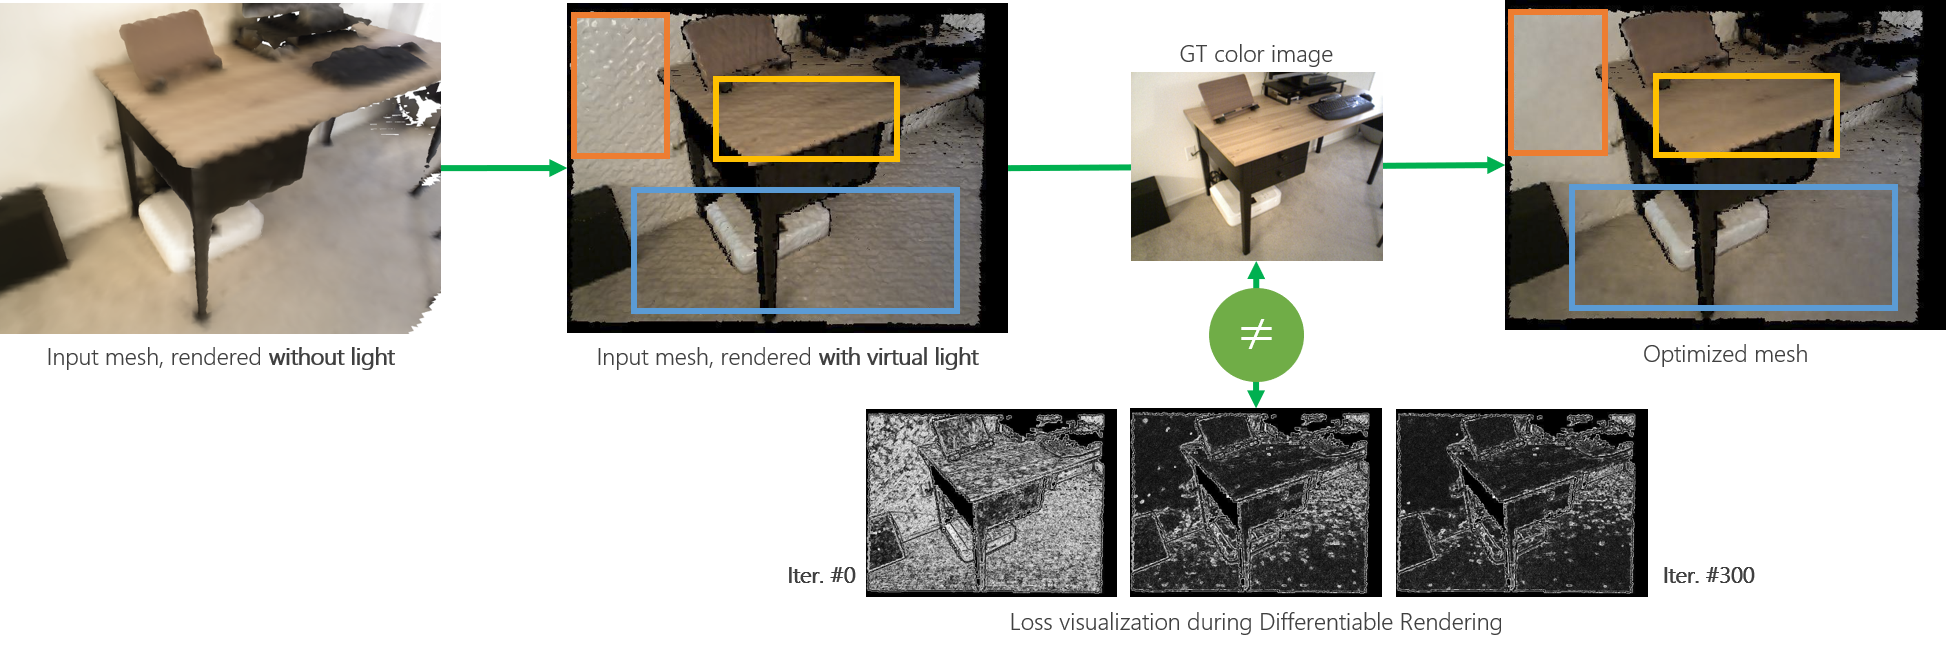
\includegraphics[width=\textwidth]{figures/0_teaser_overview_rev3.png}
    \caption{Overview of our method. (From top left) We saturate noisy vertices by rendering input TSDF mesh with virtually placed light source. We extract common-shared geometric clue between rendered input mesh and target color image. Differentiable renderer iteratively minimizes loss, which is the difference between clues from rendered input mesh and target Ground Truth color image. Orange, Yellow, and Blue inset shows difference between input mesh and optimized mesh. Our method successfully reduces noise in mesh vertices. Furthermore, our provided video shows input mesh that is being optimized (right-side of the video) as iteration continues, as well as the visualization of loss (left-side of the video) that is being minimized: \url{https://drive.google.com/file/d/10F_I89m5O-RWOIxocYoxG2QOkJc7YWlF/view?usp=sharing}}
    \label{fig:one}
\end{teaserfigure}

\begin{abstract}
Thanks to consistent evolution of SLAM (Simultaneous Localization and Mapping) and its related technologies, we can reconstruct geometric properties of where we are currently observing in real-time. Due to the limitation of current depth sensing hardware, however, we are generally able to obtain geometric features corrupted by noise. Color image is perceived as geometrically noise-free in terms of human vision-perception system, but to our best knowledge, encoding the information from Ground Truth for differentiable rendering under single view constraint is not discussed yet. In this report, we propose a bridge between the geometric information generated from color image and rendered mesh, so that differentiable renderer can optimize input i.e., noisy vertex position without any depth supervision. The key insight is that we can highlight noisy vertices by rendering mesh with virtually placed light sources. We compare our result with one of the state-of-the-art differentiable rendering method[1], and show our method outperforms previous method which requires prior depth information (silhouette image).
\end{abstract}


%
% The code below should be generated by the tool at
% http://dl.acm.org/ccs.cfm
% Please copy and paste the code instead of the example below.
%
\begin{CCSXML}
<ccs2012>
    <concept>
        <concept_id>10010147.10010371.10010396</concept_id>
        <concept_desc>Computing methodologies~Shape modeling</concept_desc>
        <concept_significance>500</concept_significance>
        </concept>
    <concept>
        <concept_id>10010147.10010371.10010387.10010392</concept_id>
        <concept_desc>Computing methodologies~Mixed / augmented reality</concept_desc>
        <concept_significance>500</concept_significance>
        </concept>
    </ccs2012>
\end{CCSXML}

\ccsdesc[500]{Computing methodologies~Shape modeling}
\ccsdesc[500]{Computing methodologies~Mixed / augmented reality}

%
% End generated code
%


\keywords{Differentiable rendering, Mesh denoising}



\maketitle

% \section{Introduction}


As a new technology, Wireless Sensor Networks (WSNs) has a wide
range of applications \cite{Akyildiz-01, Bahl-02, Culler-01}, including
environment monitoring, smart buildings, medical care, industrial and
military applications. Among them, a recent trend is to develop
commercial sensor networks that require pervasive sensing of both
environment and human beings, for example, assisted living
\cite{Akyildiz-02,CROSSBOW,Harvard-01} and smart homes
\cite{Adya-01, CROSSBOW, Harvard-01}.
% quote
\begin{quote}
  ``For these applications, sensor devices are incorporated into human
  cloths \cite{Adya-01, Bahl-02, Natarajan-01, Zhou-06} for monitoring
  health related information like EKG readings, fall detection, and
  voice recognition''.
\end{quote}
While collecting all these multimedia information
\cite{Akyildiz-02} requires a high network throughput, off-the-shelf
sensor devices only provide very limited bandwidth in a single
channel: 19.2\,Kbps in MICA2 \cite{Bahl-02} and 250\,Kbps in MICAz.

In this article, we propose MMSN, abbreviation for Multifrequency
Media access control for wireless Sensor Networks. The main
contributions of this work can be summarized as follows.
% itemize
\begin{itemize}
\item To the best of our knowledge, the MMSN protocol is the first
multifrequency MAC protocol especially designed for WSNs, in which
each device is equipped with a single radio transceiver and
the MAC layer packet size is very small.
\item Instead of using pairwise RTS/CTS frequency negotiation
\cite{Tzamaloukas-01, Adya-01, Culler-01, Zhou-06},
we propose lightweight frequency assignments, which are good choices
for many deployed comparatively static WSNs.
\item We develop new toggle transmission and snooping techniques to
enable a single radio transceiver in a sensor device to achieve
scalable performance, avoiding the nonscalable ``one
control channel + multiple data channels'' design \cite{Natarajan-01}.
\end{itemize}

% Head 1
\section{MMSN Protocol}

% Head 2
\subsection{Frequency Assignment}

We propose a suboptimal distribution to be used by each node, which is
easy to compute and does not depend on the number of competing
nodes. A natural candidate is an increasing geometric sequence, in
which
% Numbered Equation
\begin{equation}
\label{eqn:01}
P(t)=\frac{b^{\frac{t+1}{T+1}}-b^{\frac{t}{T+1}}}{b-1},
\end{equation}
where $t=0,{\ldots}\,,T$, and $b$ is a number greater than $1$.

In our algorithm, we use the suboptimal approach for simplicity and
generality. We need to make the distribution of the selected back-off
time slice at each node conform to what is shown in
Equation~\eqref{eqn:01}. It is implemented as follows: First, a random
variable $\alpha$ with a uniform distribution within the interval $(0,
1)$ is generated on each node, then time slice $i$ is selected
according to the following equation:
% Unnumbered Equation
\[
i=\lfloor(T+1)\log_b[\alpha(b-1)+1]\rfloor.
\]
It can be easily proven that the distribution of $i$ conforms to Equation
(\ref{eqn:01}).

So protocols \cite{Tzamaloukas-01, Akyildiz-01, Adya-01, Bahl-02, Culler-01,Zhou-06} that use RTS/CTS
controls\footnote{RTS/CTS controls are required to be implemented by
802.11-compliant devices. They can be used as an optional mechanism
to avoid Hidden Terminal Problems in the 802.11 standard and
protocols based on those similar to \cite{Akyildiz-01} and
\cite{Adya-01}.} for frequency negotiation and reservation are not
suitable for WSN applications, even though they exhibit good
performance in general wireless ad-hoc
networks.

% Head 3
\subsubsection{Exclusive Frequency Assignment}


In exclusive frequency assignment, nodes first exchange their IDs
among two communication hops so that each node knows its two-hop
neighbors' IDs. In the second broadcast, each node beacons all
neighbors' IDs it has collected during the first broadcast period.

% Head 4
\paragraph{Eavesdropping}

Even though the even selection scheme leads to even sharing of
available frequencies among any two-hop neighborhood, it involves a
number of two-hop broadcasts. To reduce the communication cost, we
propose a lightweight eavesdropping scheme.

\subsection{Basic Notations}

As Algorithm~\ref{alg:one} states, for each frequency
number, each node calculates a random number (${\textit{Rnd}}_{\alpha}$) for
itself and a random number (${\textit{Rnd}}_{\beta}$) for each of its two-hop
neighbors with the same pseudorandom number generator.

% Algorithm
\begin{algorithm}[t]
\SetAlgoNoLine
\KwIn{Node $\alpha$'s ID ($ID_{\alpha}$), and node $\alpha$'s
neighbors' IDs within two communication hops.}
\KwOut{The frequency number ($FreNum_{\alpha}$) node $\alpha$ gets assigned.}
$index$ = 0; $FreNum_{\alpha}$ = -1\;
\Repeat{$FreNum_{\alpha} > -1$}{
        $Rnd_{\alpha}$ = Random($ID_{\alpha}$, $index$)\;
        $Found$ = $TRUE$\;
        \For{each node $\beta$ in $\alpha$'s two communication hops
    }{
      $Rnd_{\beta}$ = Random($ID_{\beta}$, $index$)\;
      \If{($Rnd_{\alpha} < Rnd_{\beta}$) \text{or} ($Rnd_{\alpha}$ ==
          $Rnd_{\beta}$ \text{and} $ID_{\alpha} < ID_{\beta}$)\;
      }{
        $Found$ = $FALSE$; break\;
      }
        }
     \eIf{$Found$}{
           $FreNum_{\alpha}$ = $index$\;
         }{
           $index$ ++\;
     }
      }
\caption{Frequency Number Computation}
\label{alg:one}
\end{algorithm}


Bus masters are divided into two disjoint sets, $\mathcal{M}_{RT}$
and $\mathcal{M}_{NRT}$.
% description
\begin{description}
\item[RT Masters]
$\mathcal{M}_{RT}=\{ \vec{m}_{1},\dots,\vec{m}_{n}\}$ denotes the
$n$ RT masters issuing real-time constrained requests. To model the
current request issued by an $\vec{m}_{i}$ in $\mathcal{M}_{RT}$,
three parameters---the recurrence time $(r_i)$, the service cycle
$(c_i)$, and the relative deadline $(d_i)$---are used, with their
relationships.
\item[NRT Masters]
$\mathcal{M}_{NRT}=\{ \vec{m}_{n+1},\dots,\vec{m}_{n+m}\}$ is a set
of $m$ masters issuing nonreal-time constrained requests. In our
model, each $\vec{m}_{j}$ in $\mathcal{M}_{NRT}$ needs only one
parameter, the service cycle, to model the current request it
issues.
\end{description}

Here, a question may arise, since each node has a global ID. Why
don't we just map nodes' IDs within two hops into a group of
frequency numbers and assign those numbers to all nodes within two
hops?

\section{Simulator}
\label{sec:sim}

If the model checker requests successors of a state which are not
created yet, the state space uses the simulator to create the
successors on-the-fly. To create successor states the simulator
conducts the following steps.
% enumerate
\begin{enumerate}
\item Load state into microcontroller model.
\item Determine assignments needed for resolving nondeterminism.
\item For each assignment.
      \begin{enumerate}
      \item either call interrupt handler or simulate effect of next instruction, or
      \item evaluate truth values of atomic propositions.
      \end{enumerate}
\item Return resulting states.
\end{enumerate}
Figure~\ref{fig:two} shows a typical microcontroller C program that
controls an automotive power window lift. The program is one of the
programs used in the case study described in Section~\ref{sec:sim}.
At first sight, the programs looks like an ANSI~C program. It
contains function calls, assignments, if clauses, and while loops.
% Figure
\begin{figure}
  
\includegraphics{figures/mouse}
  \caption{Code before preprocessing.}
  \label{fig:two}
\end{figure}

\subsection{Problem Formulation}

The objective of variable coalescence-based offset assignment is to find
both the coalescence scheme and the MWPC on the coalesced graph. We start
with a few definitions and lemmas for variable coalescence.

% Enunciations
\begin{definition}[Coalesced Node (C-Node)]A C-node is a set of
live ranges (webs) in the AG or IG that are coalesced. Nodes within the same
C-node cannot interfere with each other on the IG. Before any coalescing is
done, each live range is a C-node by itself.
\end{definition}

\begin{definition}[C-AG (Coalesced Access Graph)]The C-AG is the access
graph after node coalescence, which is composed of all C-nodes and C-edges.
\end{definition}

\begin{lemma}
The C-MWPC problem is NP-complete.
\end{lemma}
\begin{proof} C-MWPC can be easily reduced to the MWPC problem assuming a
coalescence graph without any edge or a fully connected interference graph.
Therefore, each C-node is an uncoalesced live range after value separation
and C-PC is equivalent to PC. A fully connected interference graph is made
possible when all live ranges interfere with each other. Thus, the C-MWPC
problem is NP-complete.
\end{proof}

\begin{lemma}[Lemma Subhead]The solution to the C-MWPC problem is no
worse than the solution to the MWPC.
\end{lemma}
\begin{proof}
Simply, any solution to the MWPC is also a solution to the
C-MWPC. But some solutions to C-MWPC may not apply to the MWPC (if any
coalescing were made).
\end{proof}

\section{Performance Evaluation}

During all the experiments, the Geographic Forwarding (GF) by Akyildiz
et al.~\shortcite{Akyildiz-01} routing protocol is used. GF exploits
geographic information of nodes and conducts local data-forwarding to
achieve end-to-end routing. Our simulation is configured according to
the settings in Table~\ref{tab:one}. Each run lasts for 2 minutes and
repeated 100 times. For each data value we present in the results, we
also give its 90\% confidence interval.

% Table
\begin{table}%
\caption{Simulation Configuration}
\label{tab:one}
\begin{minipage}{\columnwidth}
\begin{center}
\begin{tabular}{ll}
  \toprule
  TERRAIN\footnote{This is a table footnote. This is a
    table footnote. This is a table footnote.}   & (200m$\times$200m) Square\\ \midrule
  Node Number     & 289\\
  Node Placement  & Uniform\\
  Application     & Many-to-Many/Gossip CBR Streams\\
  Payload Size    & 32 bytes\\
  Routing Layer   & GF\\
  MAC Layer       & CSMA/MMSN\\
  Radio Layer     & RADIO-ACCNOISE\\
  Radio Bandwidth & 250Kbps\\
  Radio Range     & 20m--45m\\
  \bottomrule
\end{tabular}
\end{center}
\bigskip\centering
\footnotesize\emph{Source:} This is a table
 sourcenote. This is a table sourcenote. This is a table
 sourcenote.

 \emph{Note:} This is a table footnote.
\end{minipage}
\end{table}%


\section{Conclusions}

In this article, we develop the first multifrequency MAC protocol for
WSN applications in which each device adopts a
single radio transceiver. The different MAC design requirements for
WSNs and general wireless ad-hoc networks are
compared, and a complete WSN multifrequency MAC design (MMSN) is
put forth. During the MMSN design, we analyze and evaluate different
choices for frequency assignments and also discuss the nonuniform
back-off algorithms for the slotted media access design.

% Start of "Sample References" section

\section{Typical References in New ACM Reference Format}
A paginated journal article \cite{Abril07}, an enumerated
journal article \cite{Cohen07}, a reference to an entire issue \cite{JCohen96},
a monograph (whole book) \cite{Kosiur01}, a monograph/whole book in a series (see 2a in spec. document)
\cite{Harel79}, a divisible-book such as an anthology or compilation \cite{Editor00}
followed by the same example, however we only output the series if the volume number is given
\cite{Editor00a} (so Editor00a's series should NOT be present since it has no vol. no.),
a chapter in a divisible book \cite{Spector90}, a chapter in a divisible book
in a series \cite{Douglass98}, a multi-volume work as book \cite{Knuth97},
an article in a proceedings (of a conference, symposium, workshop for example)
(paginated proceedings article) \cite{Andler79}, a proceedings article
with all possible elements \cite{Smith10}, an example of an enumerated
proceedings article \cite{VanGundy07},
an informally published work \cite{Harel78}, a doctoral dissertation \cite{Clarkson85},
a master's thesis: \cite{anisi03}, an online document / world wide web
resource \cite{Thornburg01, Ablamowicz07, Poker06}, a video game (Case 1) \cite{Obama08} and (Case 2) \cite{Novak03}
and \cite{Lee05} and (Case 3) a patent \cite{JoeScientist001},
work accepted for publication \cite{rous08}, 'YYYYb'-test for prolific author
\cite{SaeediMEJ10} and \cite{SaeediJETC10}. Other cites might contain
'duplicate' DOI and URLs (some SIAM articles) \cite{Kirschmer:2010:AEI:1958016.1958018}.
Boris / Barbara Beeton: multi-volume works as books
\cite{MR781536} and \cite{MR781537}.

A couple of citations with DOIs: \cite{2004:ITE:1009386.1010128,
  Kirschmer:2010:AEI:1958016.1958018}.

Online citations: \cite{TUGInstmem, Thornburg01, CTANacmart}.



% DO NOT INCLUDE ACKNOWLEDGMENTS IN AN ANONYMOUS SUBMISSION TO SIGGRAPH 2019
%\begin{acks}
%
%The authors would like to thank Dr. Maura Turolla of Telecom
%Italia for providing specifications about the application scenario.
%
%The work is supported by the \grantsponsor{GS501100001809}{National
%  Natural Science Foundation of
%  China}{http://dx.doi.org/10.13039/501100001809} under Grant
%No.:~\grantnum{GS501100001809}{61273304\_a}
%and~\grantnum[http://www.nnsf.cn/youngscientists]{GS501100001809}{Young
%  Scientists' Support Program}.
%
%
%\end{acks}

% Bibliography
\bibliographystyle{ACM-Reference-Format}
\bibliography{sample-bibliography}

% Appendix
\appendix
\section{Switching Times}

In this appendix, we measure the channel switching time of Micaz
\cite{CROSSBOW} sensor devices.  In our experiments, one mote
alternatingly switches between Channels~11 and~12. Every time after
the node switches to a channel, it sends out a packet immediately and
then changes to a new channel as soon as the transmission is finished.
We measure the number of packets the test mote can send in 10 seconds,
denoted as $N_{1}$. In contrast, we also measure the same value of the
test mote without switching channels, denoted as $N_{2}$. We calculate
the channel-switching time $s$ as
\begin{displaymath}%
s=\frac{10}{N_{1}}-\frac{10}{N_{2}}.
\end{displaymath}%
By repeating the experiments 100 times, we get the average
channel-switching time of Micaz motes: 24.3\,$\mu$s.

\section{Introduction}

To satisfy increasing demand of 
Augmented Reality (AR) technology, we required to obtain geometric information of observed real scene as precise as possible. 
As precision of geometric detail is increased, we can augment virtual objects with more consistency from computer graphics (Photorealistic Rendering) perspective, and we are able to estimate camera poses from perfect correspondences from computer vision (Simultaneous Localization and Mapping; SLAM) perspective.

Capturing detailed geometry is still remain as technical challenge due to hardware/computational limitation of SLAM. 
It is obvious that consumer-level depth sensing technology still has noisy observation. 
We can cope this by divide a real scene with less detailed (coarse) voxels to smooting out noisy depth measurements when generating TSDF mesh. 
In this way, however, it fails to retain geometric detail even in the case of reconstructing perceptually simple geometry (e.g., edge between planes).
To preserve geometric detail, we still need to divide voxels as fine as possible where is geometrically complex. 
This directly affects to rendering performance, as rendering requires primitive traversal in order to appropriately propagates lighting information for every single frame. 
Due to those limitations, we are compromised to use TSDF meshes from acceptably coarse voxels, which have geometric incorrectness including noise. 
Nevertheless, there is strong demand to perfect geometry captured from SLAM sequences. 

Recent advances of Differentiable Rendering make it possible to optimize current input parameters by observing a set of given Ground Truth images. 
This seems promising to SLAM, as they naturally capture Ground Truth color images whereas generating input TSDF mesh corrupted by noisy measurements. 
However, it is unclear that how to interpret (perceptually encoded) geometric clues within color images, reflect those information into actual geometry to minimize its imperfection. 
Moreover, there is some limitations hinder directly applying previous differentiable rendering techniques into SLAM dataset. 
We explained such difficulties in (Fig. \ref{fig:difference_simple_mesh_and_tsdf_mesh}).

Our main contribution is bridging the gap between perceptional noise-free geometric features from input color image and noisy geometric feature in input mesh. 
To exploit this, we interpreted input color image as a result of perfect renderer with perfect geometry. 
Under certain assumptions, we argued that radiance is consistent if a point and its neighbors are lie on a same plane.
Generally, it is not true for virtually rendered image with input mesh, as the mesh is composed with noisy vertices.
Therefore, we optimized input mesh to have radiance consistency i.e., noise-free geometry which is input color image have.

% \PJ{TODO: move this into method; this is not our main contribution, rather it is close to implementation detail.}
% To exploit this, we borrow a novel concept of image denoising using flashlight. Images taken with flashlight can hold additional features which are hard to detect from general geometric feature (e.g., depth, normal etc). 
% For example, in \cite{eisemann2004flash} \cite{petschnigg2004digital} flashy photography is used to enhance images taken from scene which has insufficient lighting condition. 
% \cite{moon2013robust} is pioneering work that adopt image enhancement using flashlight on photorealistic rendering domain, by casting virtual flashlights to capture a scene’s reflective / refractive features, which are not stored in traditional G-buffers. 
% Based on these approaches, we saturate noisy vertices by casting virtual light, which are never detected when rendered with mesh’s albedo only. 
% Please refer the leftmost image (rendered without light) and its connected image (rendered with virtual light) in \ref{fig:teaser} for details. 
We demonstrate our results, compare with result from previous method, and show that our method outperforms previous result.
\section{Previous Works}

\paragraph{TSDF Mesh Noise Reduction in SLAM}
Starting from pioneering work [5], 
estimating true depth from noisy measurements 
has been one of the major challenges in SLAM. 
Basically, [5] first introduced the definition of ‘fusion’, 
which is accumulating noisy world positions into a voxel. 
This acts as similar with spatial running average filter, 
therefore it is known that accumulating frames 
that captures same region can reduce noise incrementally. 
However, this takes a lot of time to converge depth values 
to a true mean, which interferes practical AR application experience. 
Therefore, various depth noise reduction techniques are applied to SLAM systems, 
including simple bilateral filter [6],  merging depth information of neighboring frames either offline [7][8], or online [9][10]. 
All mentioned previous works require multiple depth frames 
in order to generate reliable mesh which takes a long time, 
and they did not consider color images, which holds perceptive geometric information. 
Our method, in contrast, is able to infer geometric clue in color image, 
thus able to de-noise input mesh without multiple frames.

\paragraph{Differentiable Rendering}
Differentiable rendering is the technique that 
optimizing input parameters by observing a set of target images 
via iteratively render a scene with current state of input parameters (i.e., forward pass), 
as well as propagate gradients along with computation graph (i.e., backward pass) built at forward pass. 
Due to the fact that it does not require any prior knowledge (e.g., pre-trained model trained from external dataset) 
other than target images, this seems an off-the-shelf optimizer for SLAM 
since we naturally capture target image during scanning process, 
whereas fused mesh is contaminated with noise due to its nature limitations. 
However, there are ambiguities that have to be considered 
in order to adapt differentiable rendering to optimize SLAM problems. 
Figure 2. describes the different setup between simple mesh optimization 
and indoor TSDF mesh optimization. 
Our method bypasses those ambiguities via inferring geometric clue 
without necessity of silhouette information, as well as multiple target observations.
\begin{figure}
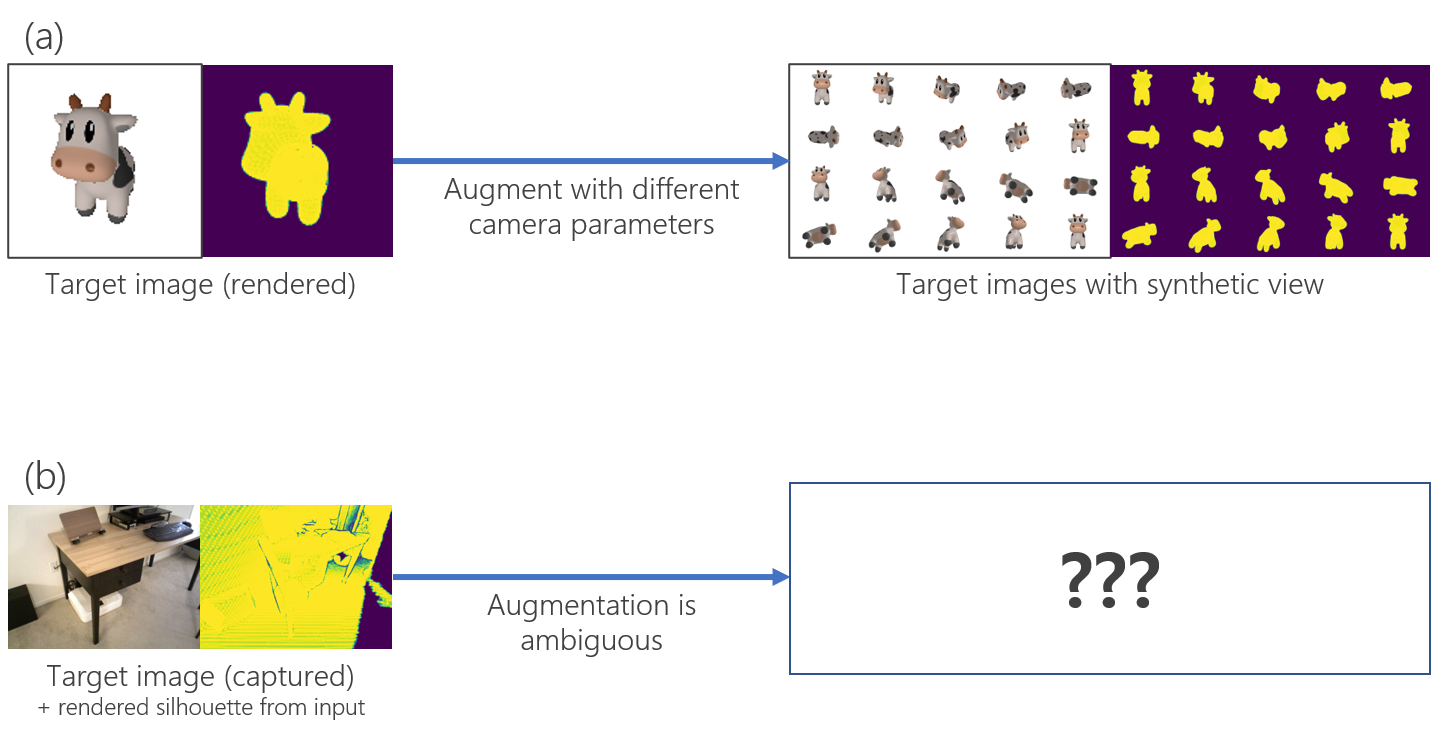
\includegraphics[width=\columnwidth]{figures/2_prev_difference_simple_mesh_and_tsdf_mesh.png}
\caption{Different setup between optimizing simple mesh and TSDF mesh from SLAM. Previous works aimed to optimize input geometry to set of target images captured with different camera view either synthetically[11][12][13][14] or by taking calibrated real photographs[14]. However, in the case of TSDF mesh from SLAM it is ambiguous since (1) input is not separated with its backgrounds, hence silhouette image is hard to generate (2) we cannot generate synthetic target views (3) it is hard to sample real images from SLAM sequences which captures a region that input mesh represents, since the labeled camera pose paired with target image is estimated value. It is well-known that camera poses from SLAM is inaccurate. (a) It is straightforward to generate synthetic target images if the target image can be rendered. (b) Unlike (a), it is much hard to augment target images in order to optimize indoor TSDF mesh.}
\label{fig:two}
\end{figure}


\end{document}
